\chapter{Cut and count and ML comparison (Temp title)}
\label{sec:results}
Now we have looked at how .........................
%\input{Sections/Results/CutAndCount/SlepSlep}
%%\section{Cut and count}
%\label{sec:resultsCandC}

\input{Sections/Results/CutAndCount/SlepSlep}




\input{Sections/Results/CutAndCount/C1C1_WW}

\input{Sections/Results/CutAndCount/Mono-Z}

%\section{Machine learning}
\label{sec:resultsML}

\subsection{BDT}
\label{sec:resultsBDT}

\subsubsection{MC simulated data}

\subsubsection{Real data}




\subsection{Neural networks}
\label{sec:resultsNN}

\subsubsection{MC simulated data}

\subsubsection{Real data}

\section{Quantifying the sensitivity}
\label{sec:significance}

The overall goal with the analysis carried out in this thesis is to optimize the sensitivity to discover new physics and possibly in the end to claim discovery of new particles. To check if we have succeeded in making our model sensitive to new physics we can check the expected p-values and significances for our signal region. 

Each event in the data will either pass or fail the cuts defining the signal region used in the analysis. The number of events therefore follows a binomial distribution, and the probability of finding $n$ events in our region is given by equation \ref{eq:pval1}. 

\begin{equation}
    \label{eq:pval1}
    P(n|N, p) = \frac{N!}{n!(N-n)!} p^n(1-p)^{N-n},
\end{equation}

where $N$ is the number of total events and p is the probability for the event to pass the cuts. If the number of total events gets very big and the probability $p$ gets very small, we can approximate equation \ref{eq:pval1} as a Poisson distribution, which is given by

\begin{equation}
    \label{eq:pval2}
    P(n|\nu) = \frac{\nu^n}{n!} e^{-\nu},
\end{equation}

where $\nu$ is given by a hypothesis. This equation (eq. \ref{eq:pval2}) gives us a probability of $n$ observed events when the expectation is to observe $\nu$ events. 

When we are talking about hypotheses in this thesis, we are talking about \textit{background-only} (b-only) and \textit{signal + background} (s+b) hypotheses. The b-only hypothesis is the SM, which is a well known theory. We are going to check this against the s+b hypothesis which in our case will be one of the three SUSY processes or the mono-Z process. This gives us the opportunity to introduce the p-values. A p-value is a measure to judge the deviation of the observed number of events from the b-only hypothesis expectations. If we assume that only the SM processes contribute we can use the p-value to get the probability of observing as many, or more, events as we can find in the data. With a perfectly known background the p-value can be found by

\begin{equation}
    \label{eq:pvalues}
    p = \sum_{n=n_{obs}}^\infty f(n;b),
\end{equation}


where $f(n;b)$ is the Poisson distribution given in equation \ref{eq:pval2}. It is common to convert the p-value into an observed significance $z$ with a unit Gaussian $\Phi$. This is given by

\begin{equation}
    \label{eq:signifobs}
    z = \Phi^{-1}(1-p)
\end{equation}

 and the unit is expressed with a $\sigma$ as in number of standard deviations from the center of the Gaussian distribution. To claim discovery of a new particle we need an observed significance above 5 $\sigma$. We are not going to check the observed significance in this thesis, but calculate the expected significance to see if there is any hope to discover new physics for the models we are looking at. The expected significance is the significance associated with the median number of expected events under the s+b hypothesis. It gives us a number on how well the two hypotheses we are looking at are separated. This is given by equation \ref{eq:signif}, where the p-value now is expressed as a \textit{confidence level} (CL) given as
 
 \begin{equation}
    \label{eq:CL}
    CL_{s+b} = \sum_{n=0}^{q_{obs}} \frac{(s+b)^n}{n!} e^{-(s+b)},
 \end{equation}

where $q_{obs}$ is the number of observed events. If the $CL_{s+b}$ is below 5\% we exclude that we can find any new physics with the selection criteria we have given it. Putting equation \ref{eq:signifobs} and \ref{eq:CL} together we get the expression

\begin{equation}
    \label{eq:signif}
    Z_N = \Phi^{-1}(1-CL_{s+b}),
\end{equation}

where $Z_N$ is the expected significance. To claim exclusion in the signal region we need a $CL_{s+b} \leq$ 5\% which corresponds to $Z_N \leq 1.64 \sigma$. In this thesis the $Z_N$ is calculated by an already existing tool in ROOT called \texttt{RooStats.NumberCountingUtils.BinomialExpZ} which simply takes the number of events for both background and signal as input together with a fractional background uncertainty of e.g. 20\%.







\begin{comment}

\begin{equation}
    \label{eq:pval3}
    p = P(n \geq q_{obs}|b) \sum_{n=q_{obs}}^\infty \frac{b^n}{n!} e^{-b}
\end{equation}

As mentioned several times in this project the goal is to claim discovery of the Higgs boson. To do that we have to reject the b-only hypothesis. To do this we are going to use p-values and confidence levels. \\


which is a probability of finding $n$ events in our signal region. 









\textbf{P-values}\\
Assuming a null hypothesis to be true we can use the p-value as a function that quantifies how often we would obtain data as far away from the null hypothesis as the observed data. Since it is a function of the data, the p-value is of course a random variable. We have the p-values $p_0$ and $p_1$ for the hypotheses $H_0$ and $H_1$ which is given by 

\begin{equation}
    \label{eq:p0}
    p_0 = \int_{t_{obs}}^{+ \infty} g(t|H_0) dt,
\end{equation}
and
\begin{equation}
    \label{eq:p1}
    p_1 = \int_{t_{obs}}^{+ \infty} g(t|H_1) dt.
\end{equation}

These are probabilities to find the test statistic ($t$) values that are equal or greater than the observed test statistic ($t_{obs}$). The p-values can also be expressed by confidence levels as

\begin{equation}
    \label{eq:p0CL}
    p_0 = 1-CL_b
\end{equation}
and 
\begin{equation}
    \label{eq:p1CL}
    p_1 = CL_{s+b}.
\end{equation}

How to calculate the $CL_b$ and $CL_{s+b}$ is shown in equation \ref{eq:CLb} and \ref{eq:CLsb} later in this section.\\

\textbf{Confidence levels}\\
The method we are using to check if this is a good fit is confidence levels. The confidence level tells us how often the results will fit the expectations. E.g. a confidence level of 90\% tells us that the results fit the expectations 90\% of the time. In figure \ref{fig:CL} we can see an illustrative plot of the test statistic distribution with the confidence levels marked. 


\begin{figure}[H]
    \centering
    \includegraphics[width = 0.7\textwidth]{Figures/CL.png}
    \caption{This is a illustration of the test statistic distribution for the b-only and s+b hypotheses with the $CL_b$ and $CL_{s+b}$ marked. \cite{datanal}}
    \label{fig:CL}
\end{figure}

The compability of the observed test statistic, $t_{obs}$, with the two hypothesis, b-only and s+b, are defined as

\begin{equation}
    \label{eq:CLb}
    1 - CL_b = \int_{-\infty}^{t_{obs}} \text{g(t; b-only) dt}
\end{equation}

and

\begin{equation}
    \label{eq:CLsb}
    CL_{s+b} = \int_{t_{obs}}^{+\infty} \text{g(t; s+b) dt}.
\end{equation}



\textbf{Results for the p-values and confidence levels}\\
By using equation \ref{eq:CLb} and \ref{eq:CLsb} we get the following results



In table \ref{tab:CLZ} we can see the results for the p-values ($1-CL_b$) and the confidence levels. As we can see is the expected significance is below 5$\sigma$ so we did not expect to claim a discovery which also is compatible with the observed significance from the data. \\

We can also see that the value for $CL_{s+b}$ for the b-only hypothesis is below 0.05 which is the limit for excluding this hypothesis but since the observed value is $> 0.05$ we can't exclude it either.  



\begin{table}[H]
    \centering
    \begin{tabular}{c c c}\hline
     & 1-CL_b & CL_{s+b}\\\hline\hline
    b-only     &  & \\
    s+b     &  &\\
    data &  & \\\hline
    \end{tabular}
    \caption{Caption}
    \label{tab:CL}
\end{table}


\begin{table}[H]
    \centering
    \begin{tabular}{c c}\hline
     & CL$_{s+b}$ \\\hline\hline
    Median s+b experiment     &  0.500\\
    Median b-only experiment     & 0.023\\
    Data & 0.843\\\hline
    \end{tabular}
    \caption{Caption}
    \label{tab:my_label}
\end{table}


\end{comment}

\section{Direct slepton production}
\label{sec:resSlepSlep}
\begin{figure}[H]
    \centering
    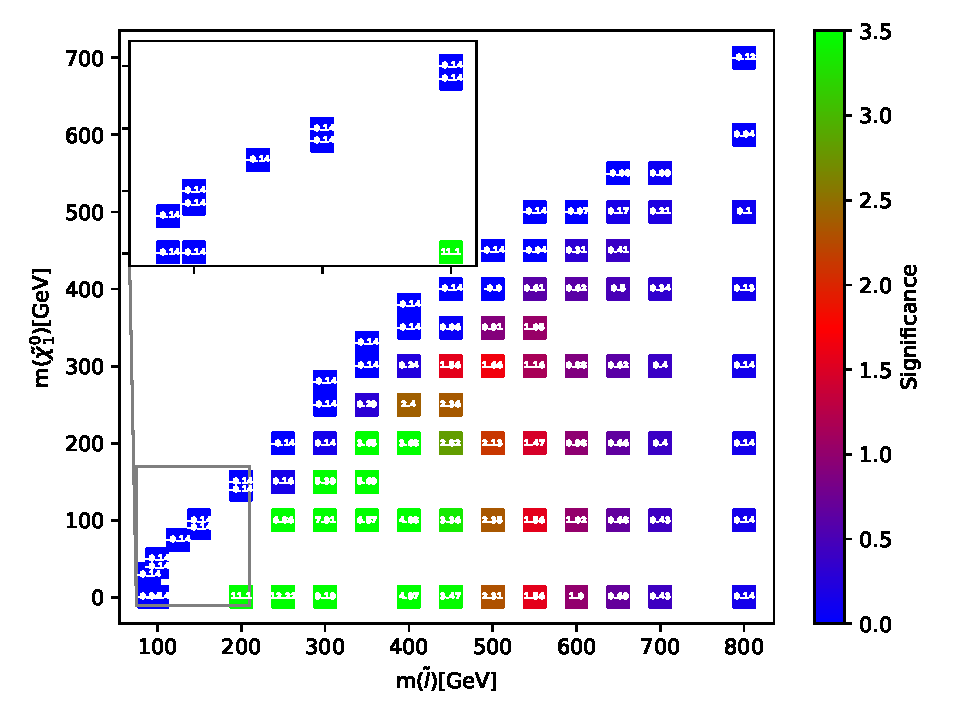
\includegraphics[width = \textwidth]{Figures/Significances/significanceCutandCount_slepslep_all.pdf}
    \caption{Caption}
    \label{fig:my_label}
\end{figure}

\begin{figure}
    \centering
    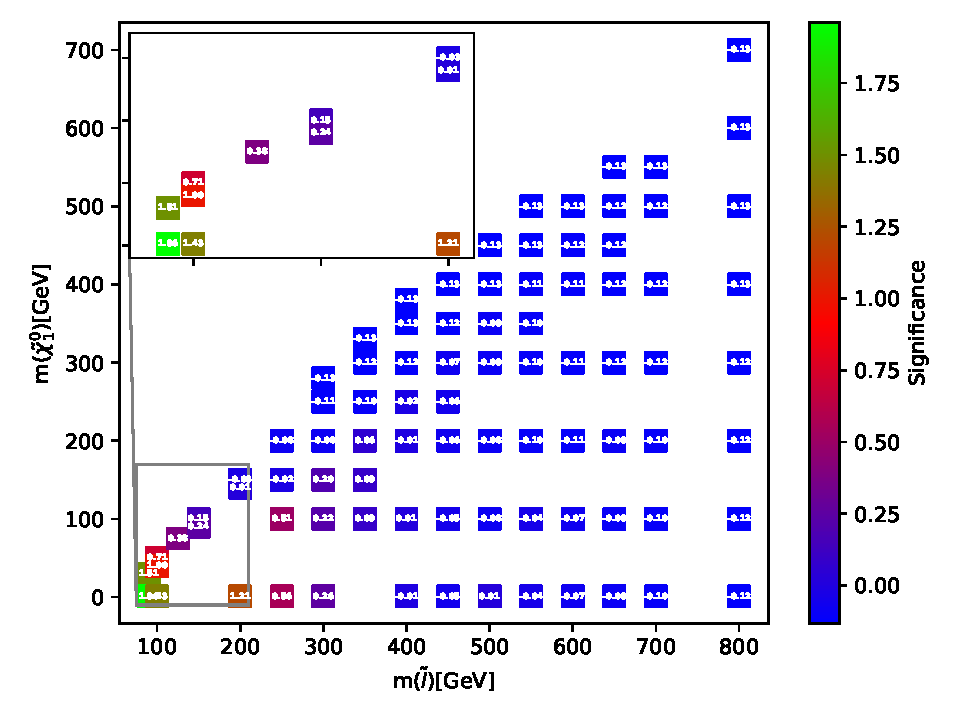
\includegraphics[width = \textwidth]{Figures/Significances/significance_BDT_slepslep_All_level.pdf}
    \caption{Caption}
    \label{fig:my_label}
\end{figure}

\begin{figure}
    \centering
    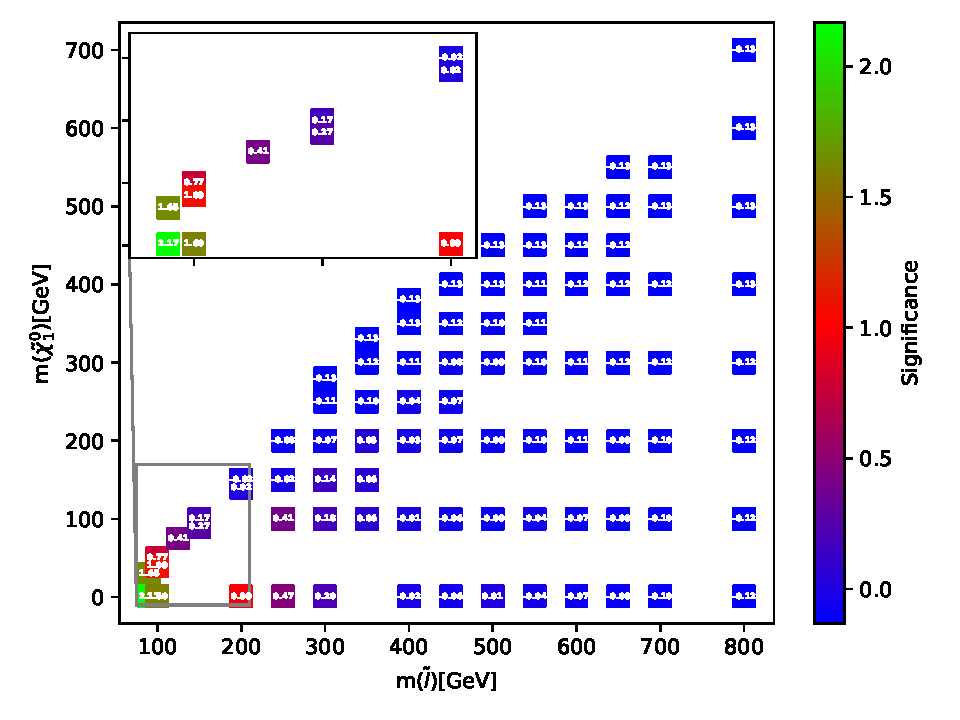
\includegraphics[width = \textwidth]{Figures/Significances/significance_BDT_slepslep_Low_level.pdf}
    \caption{Caption}
    \label{fig:my_label}
\end{figure}


\begin{figure}
    \centering
    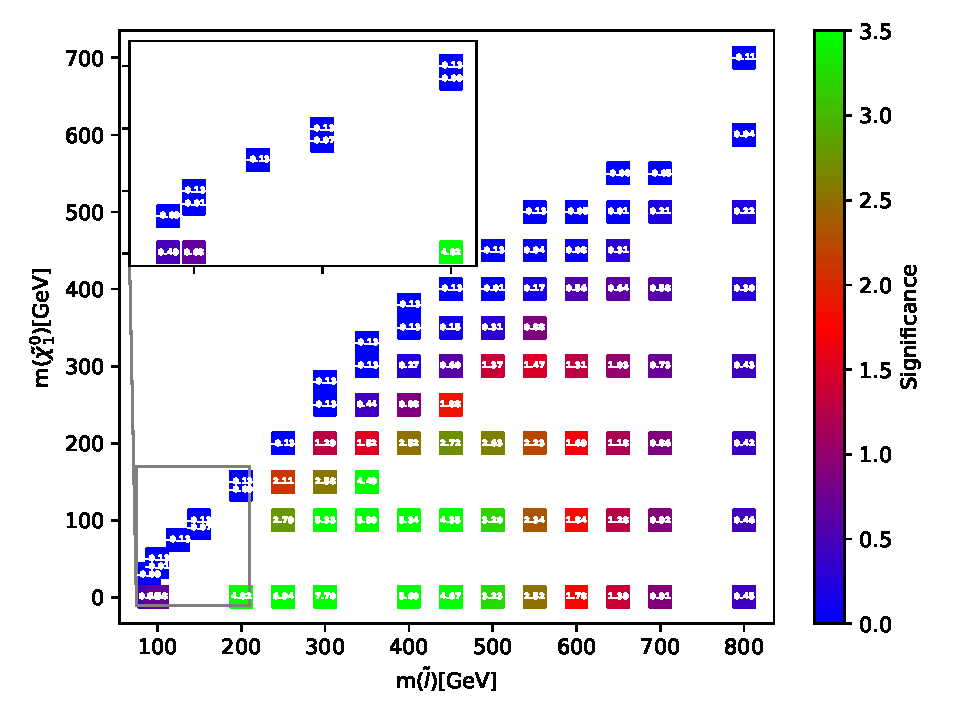
\includegraphics[width = \textwidth]{Figures/Significances/significance_BDT_slepslep_High_level.pdf}
    \caption{Caption}
    \label{fig:my_label}
\end{figure}



\begin{figure}
    \centering
    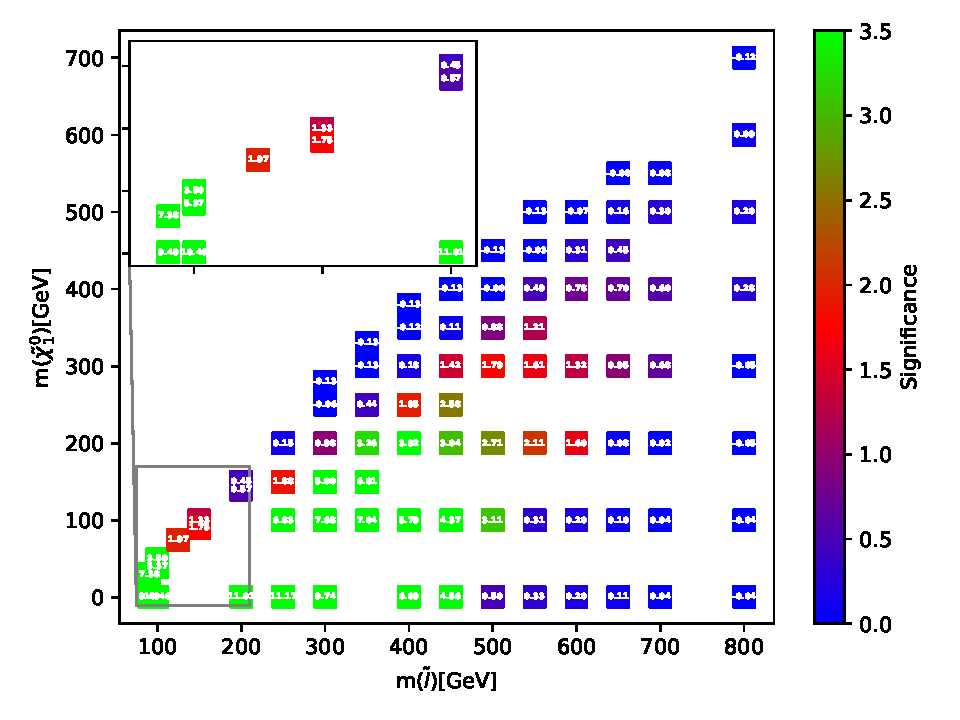
\includegraphics[width = \textwidth]{Figures/Significances/significance_NN_slepslep_All_level.pdf}
    \caption{Caption}
    \label{fig:my_label}
\end{figure}

\begin{figure}
    \centering
    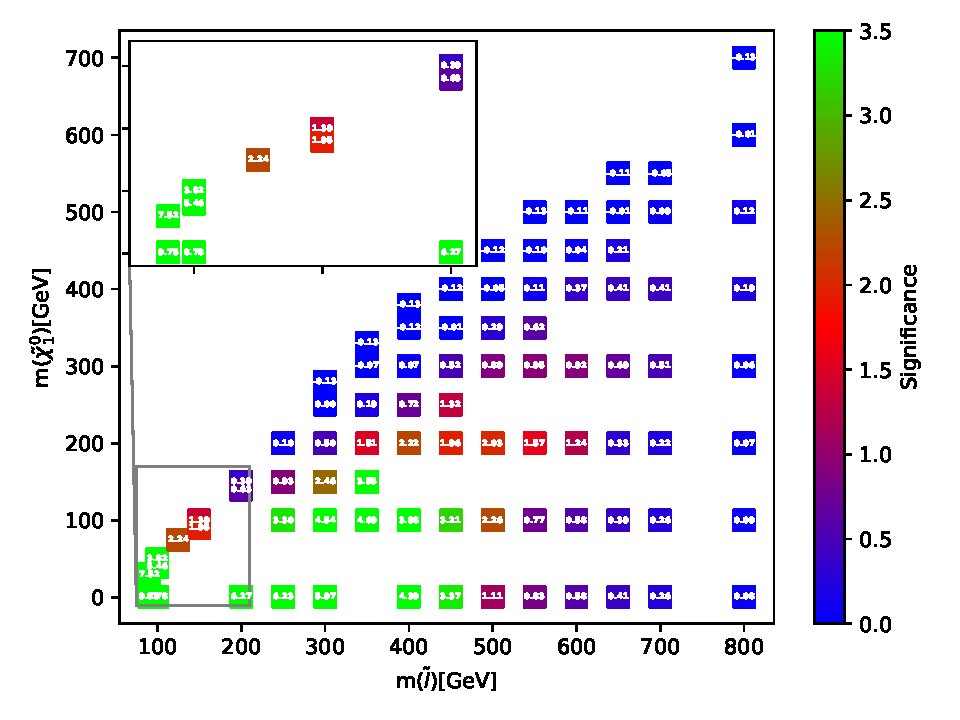
\includegraphics[width = \textwidth]{Figures/Significances/significance_NN_slepslep_Low_level.pdf}
    \caption{Caption}
    \label{fig:my_label}
\end{figure}


\begin{figure}
    \centering
    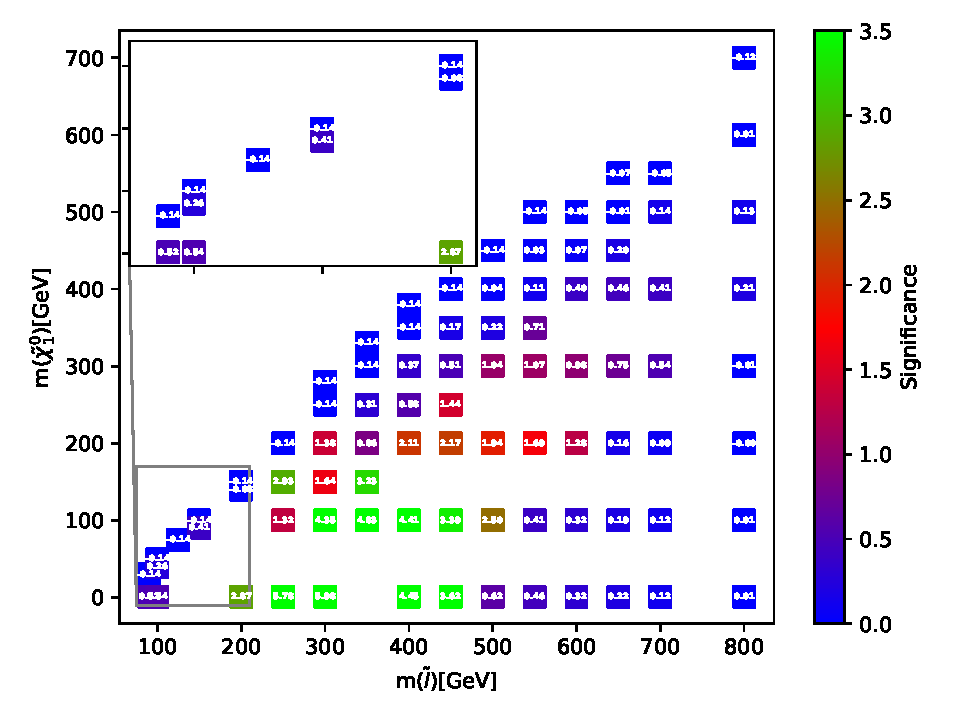
\includegraphics[width = \textwidth]{Figures/Significances/significance_NN_slepslep_High_level.pdf}
    \caption{Caption}
    \label{fig:my_label}
\end{figure}















\section{Chargino pair via slepton or sneutrino}
\label{sec:resC1C1_SlepSnu}

\begin{figure}[H]
    \centering
    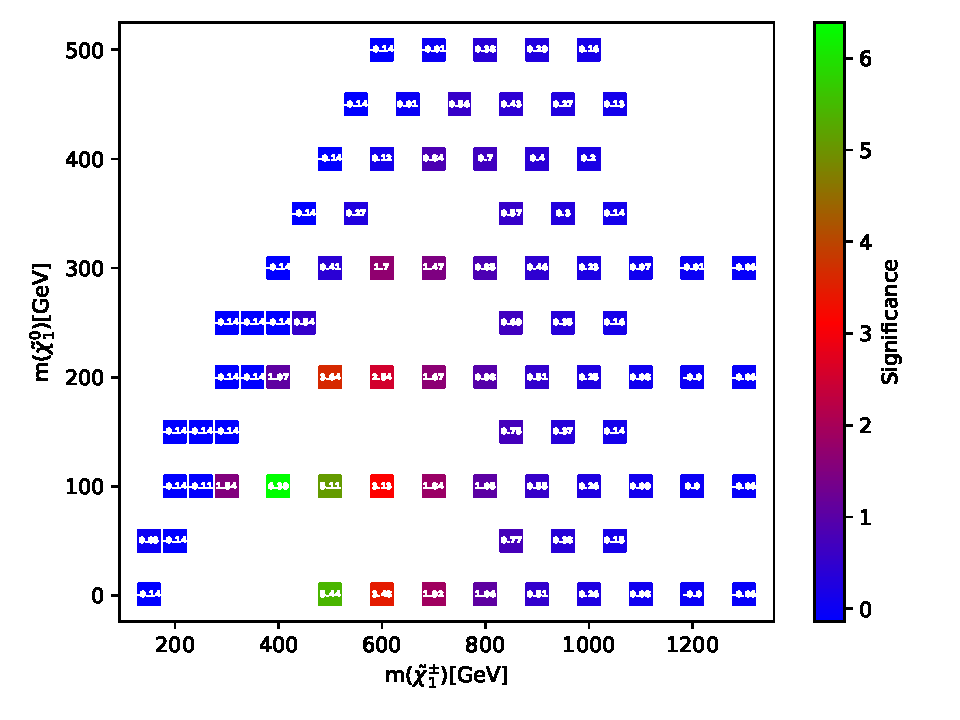
\includegraphics[width = \textwidth]{Figures/Significances/significanceCutandCount_slepsnu_all.pdf}
    \caption{Caption}
    \label{fig:my_label}
\end{figure}





\begin{figure}
    \centering
    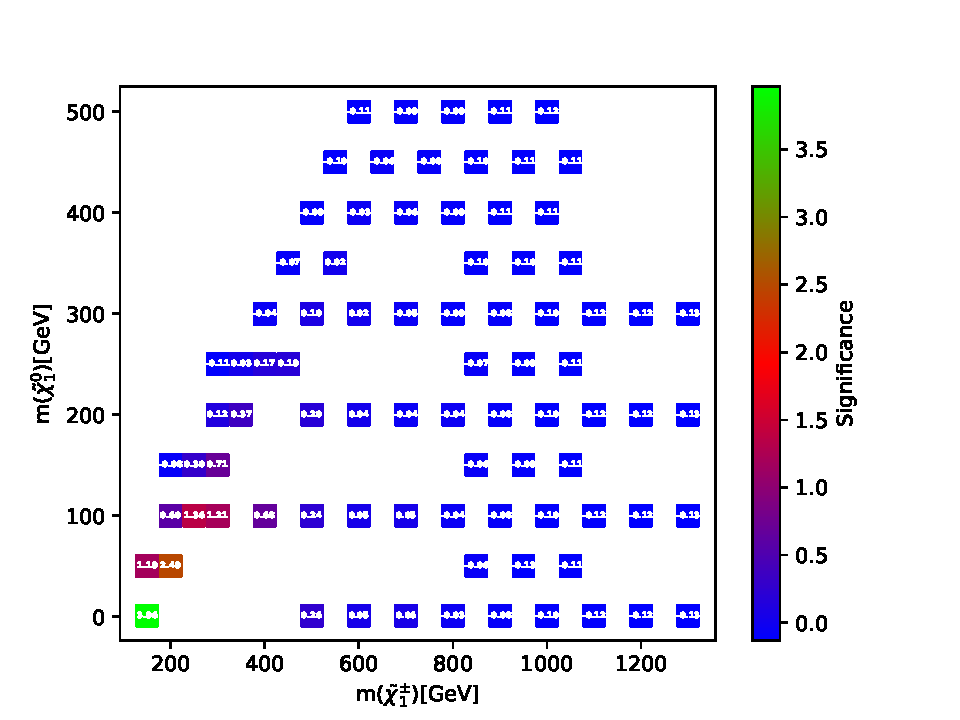
\includegraphics[width = \textwidth]{Figures/Significances/significance_BDT_slepsnu_All_level.pdf}
    \caption{Caption}
    \label{fig:my_label}
\end{figure}

\begin{figure}
    \centering
    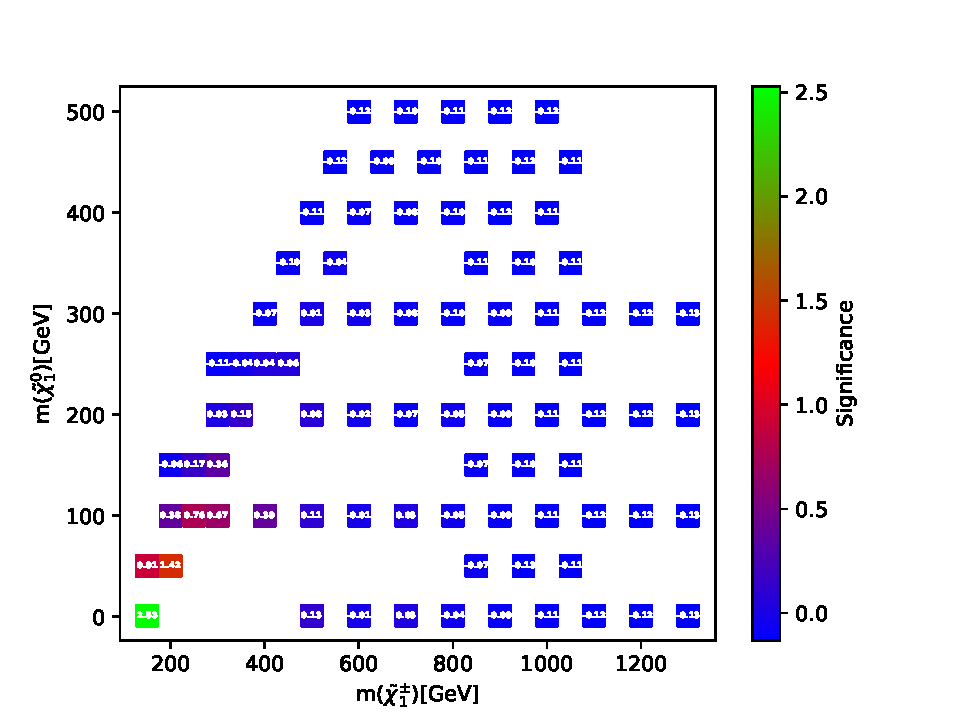
\includegraphics[width = \textwidth]{Figures/Significances/significance_BDT_slepsnu_Low_level.pdf}
    \caption{Caption}
    \label{fig:my_label}
\end{figure}


\begin{figure}
    \centering
    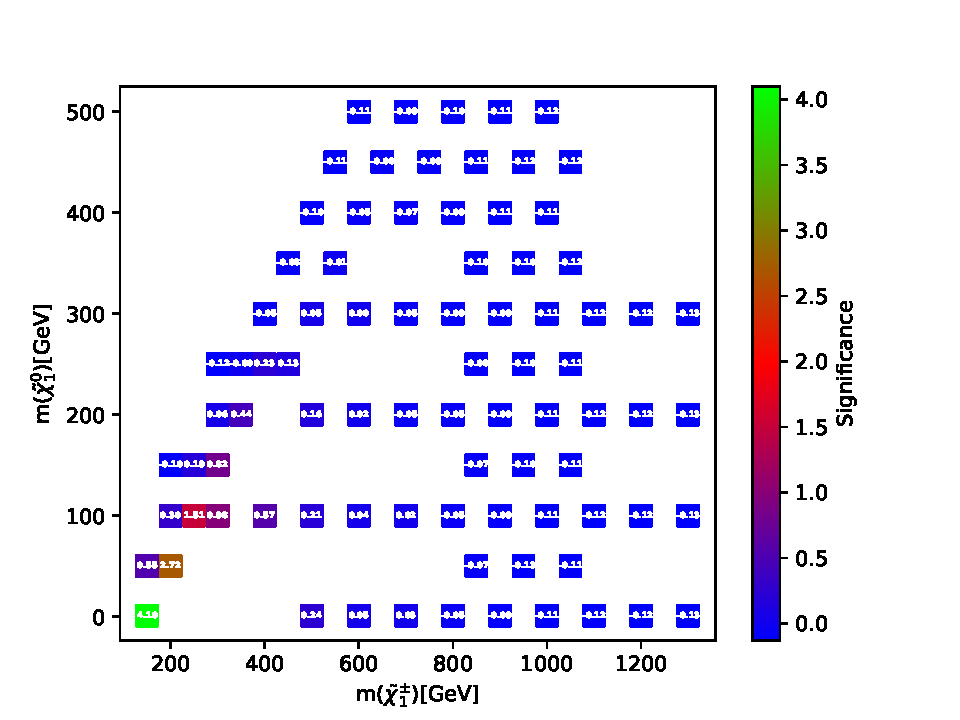
\includegraphics[width = \textwidth]{Figures/Significances/significance_BDT_slepsnu_High_level.pdf}
    \caption{Caption}
    \label{fig:my_label}
\end{figure}



\begin{figure}
    \centering
    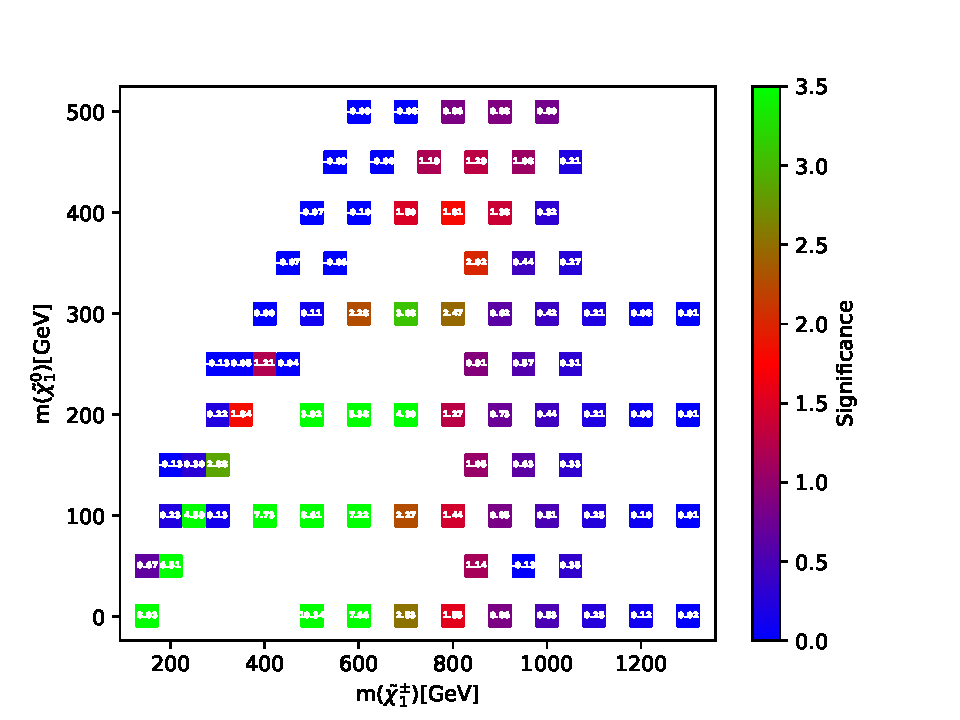
\includegraphics[width = \textwidth]{Figures/Significances/significance_NN_slepsnu_All_level.pdf}
    \caption{Caption}
    \label{fig:my_label}
\end{figure}

\begin{figure}
    \centering
    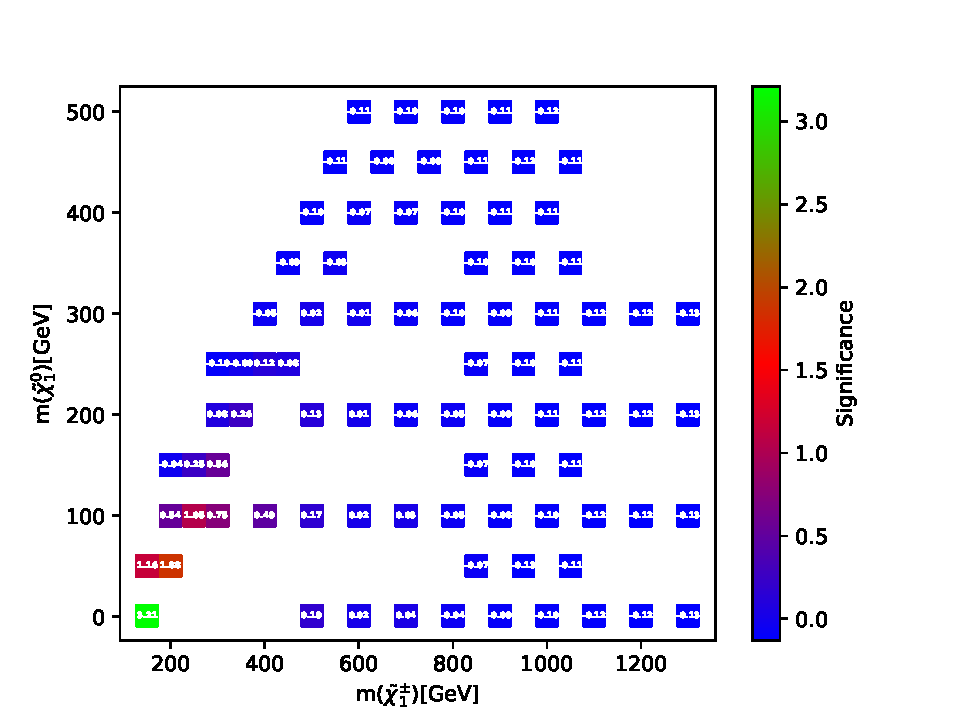
\includegraphics[width = \textwidth]{Figures/Significances/significance_NN_slepsnu_Low_level.pdf}
    \caption{Caption}
    \label{fig:my_label}
\end{figure}


\begin{figure}
    \centering
    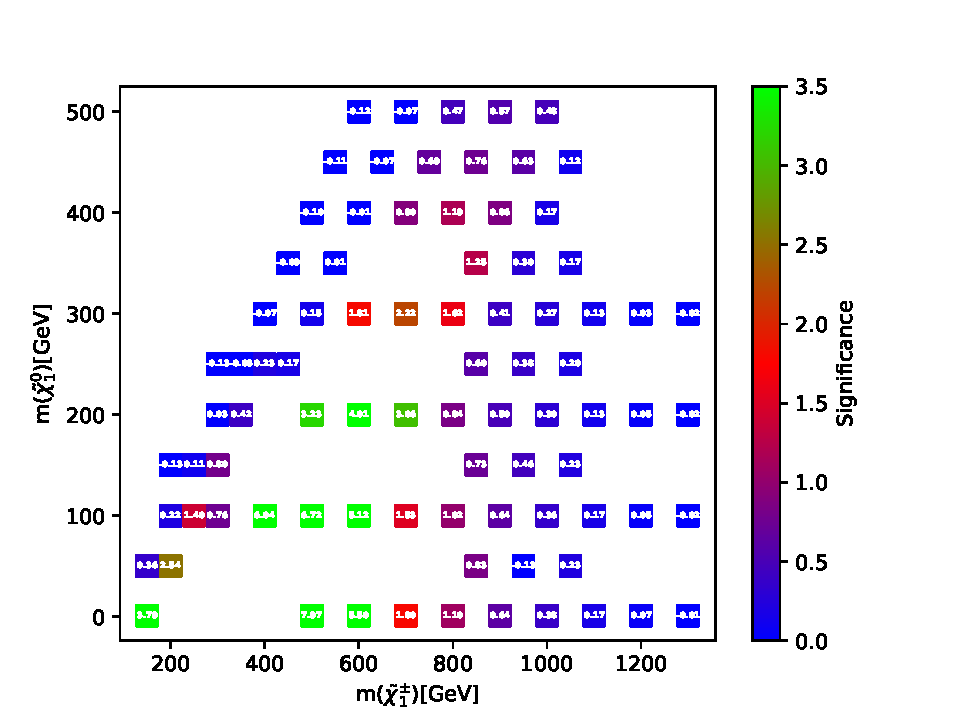
\includegraphics[width = \textwidth]{Figures/Significances/significance_NN_slepsnu_High_level.pdf}
    \caption{Caption}
    \label{fig:my_label}
\end{figure}

























\section{Chargino pair via W-bosons}
\label{sec:resC1C1_WW}
\begin{figure}[H]
    \centering
    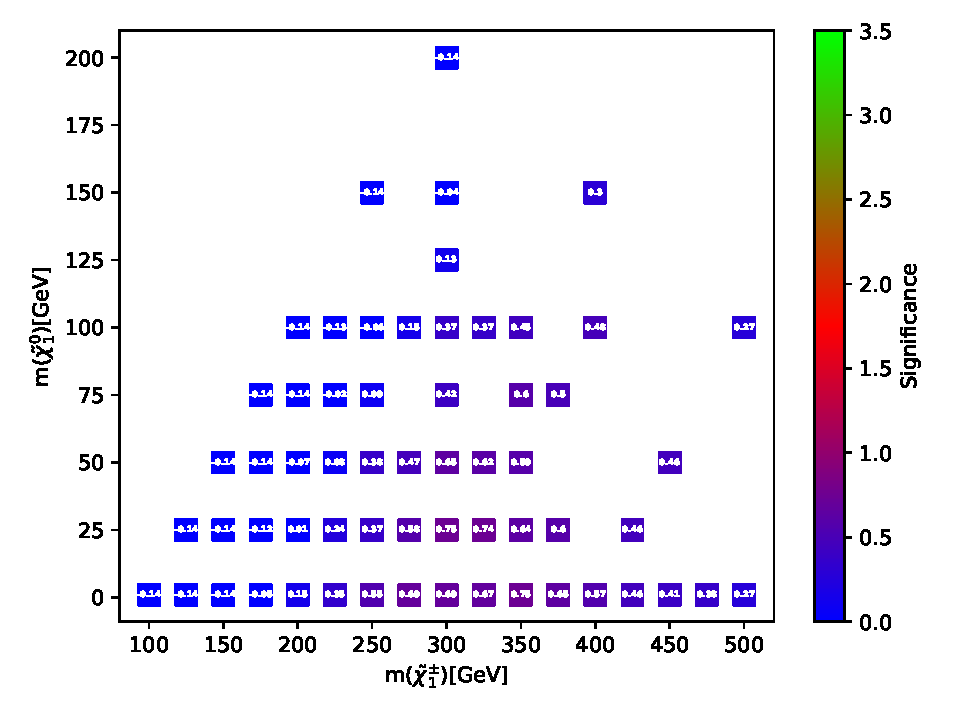
\includegraphics[width = \textwidth]{Figures/Significances/significanceCutandCount_WW_all.pdf}
    \caption{Caption}
    \label{fig:my_label}
\end{figure}



\begin{figure}
    \centering
    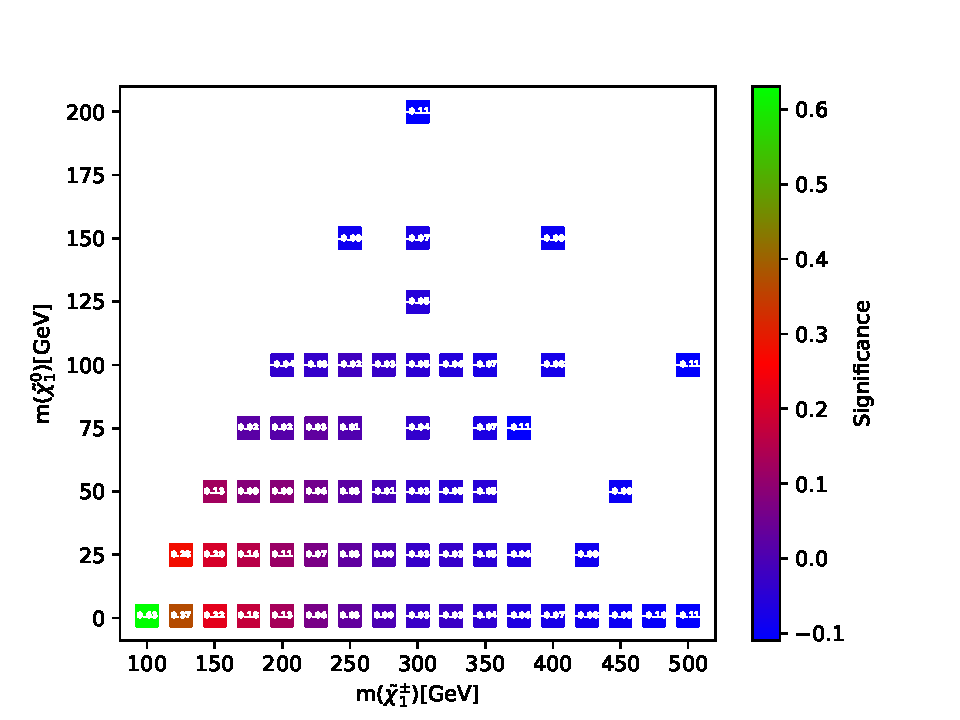
\includegraphics[width = \textwidth]{Figures/Significances/significance_BDT_WW_All_level.pdf}
    \caption{Caption}
    \label{fig:my_label}
\end{figure}

\begin{figure}
    \centering
    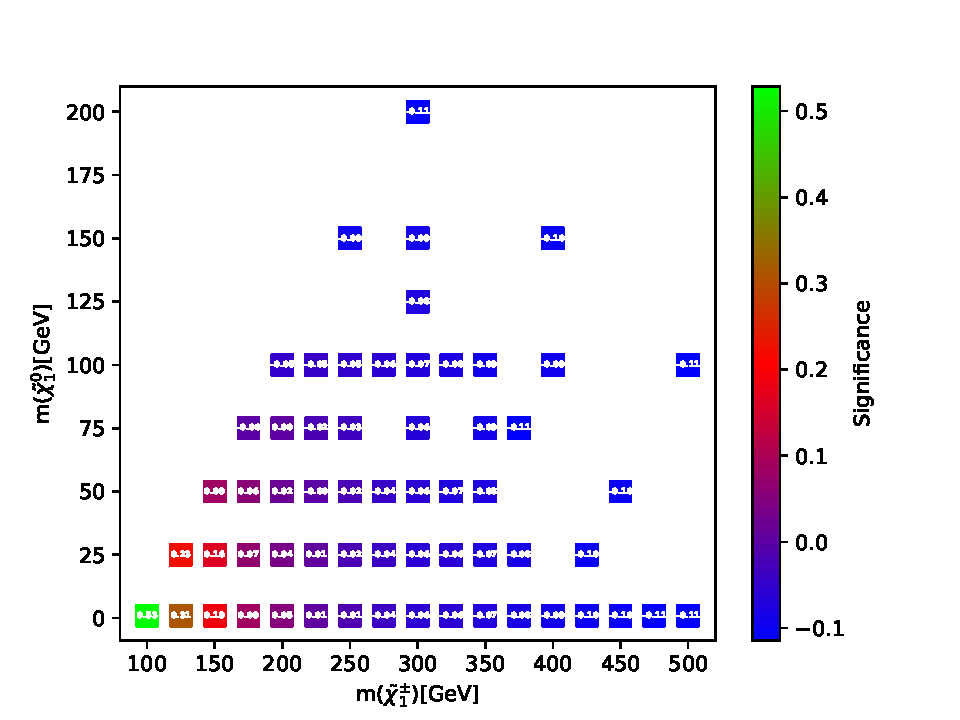
\includegraphics[width = \textwidth]{Figures/Significances/significance_BDT_WW_Low_level.pdf}
    \caption{Caption}
    \label{fig:my_label}
\end{figure}


\begin{figure}
    \centering
    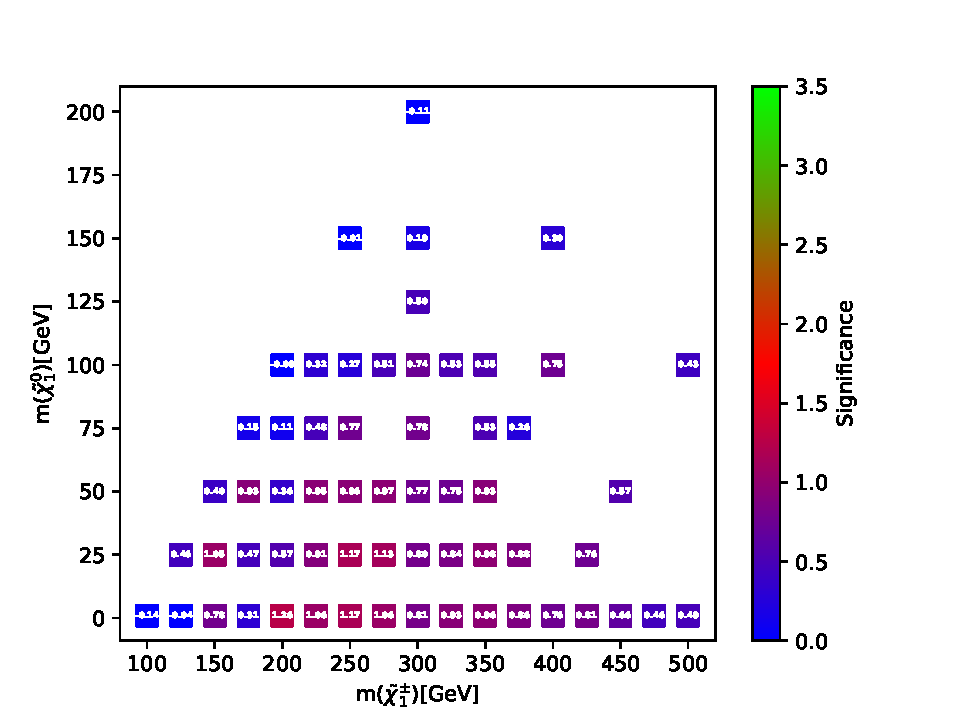
\includegraphics[width = \textwidth]{Figures/Significances/significance_BDT_WW_High_level.pdf}
    \caption{Caption}
    \label{fig:my_label}
\end{figure}



\begin{figure}
    \centering
    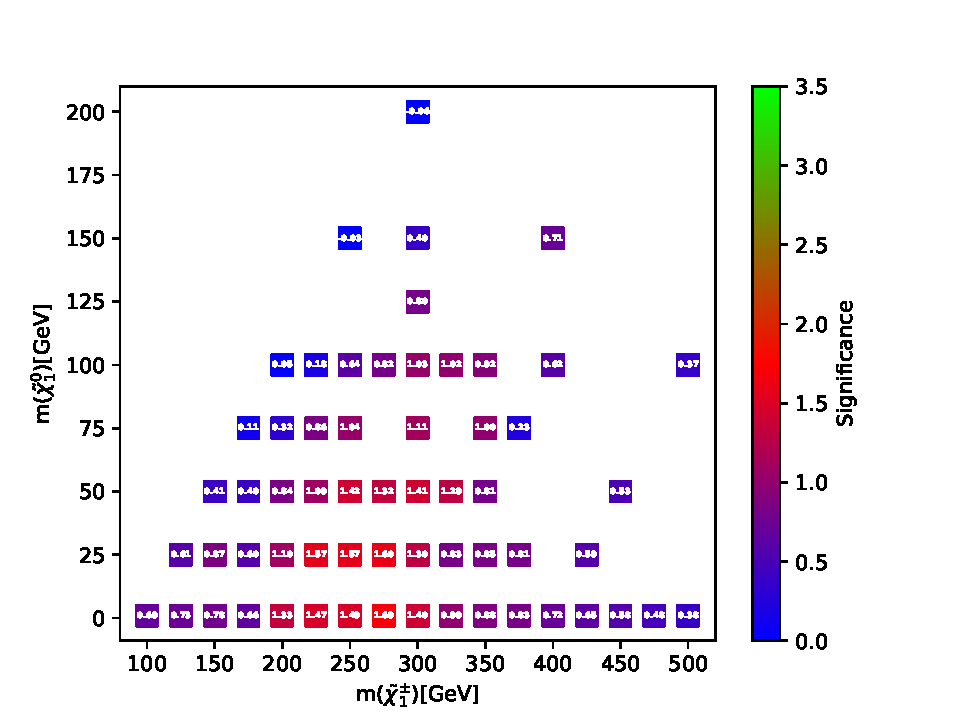
\includegraphics[width = \textwidth]{Figures/Significances/significance_NN_WW_All_level.pdf}
    \caption{Caption}
    \label{fig:my_label}
\end{figure}

\begin{figure}
    \centering
    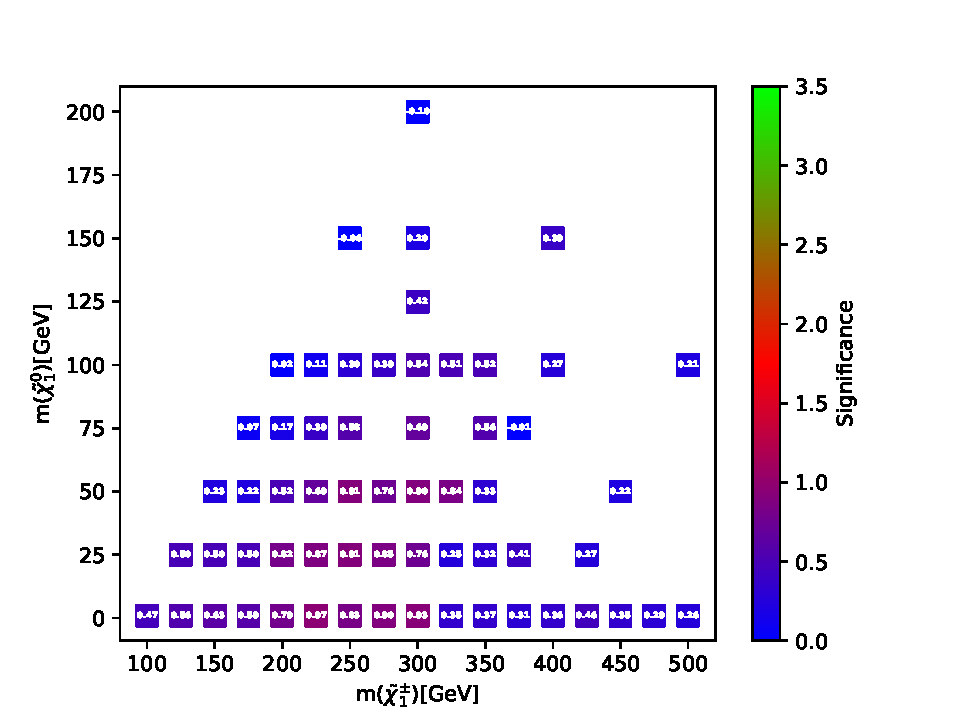
\includegraphics[width = \textwidth]{Figures/Significances/significance_NN_WW_Low_level.pdf}
    \caption{Caption}
    \label{fig:my_label}
\end{figure}


\begin{figure}
    \centering
    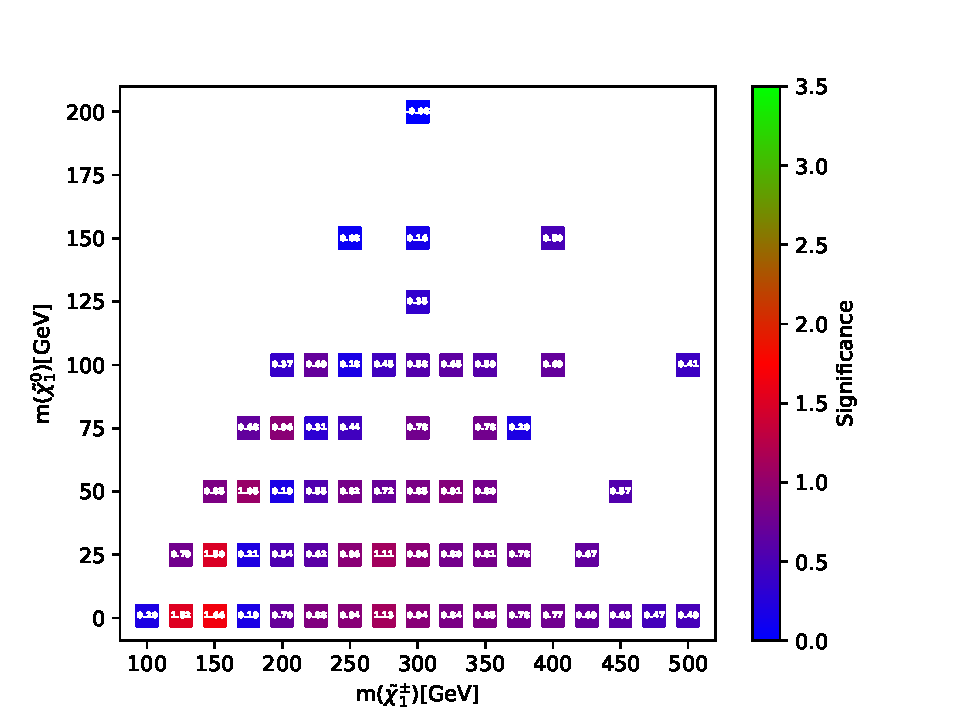
\includegraphics[width = \textwidth]{Figures/Significances/significance_NN_WW_High_level.pdf}
    \caption{Caption}
    \label{fig:my_label}
\end{figure}























\section{Mono-Z}
\label{sec:resMono-Z}
\begin{figure}[H]
    \centering
    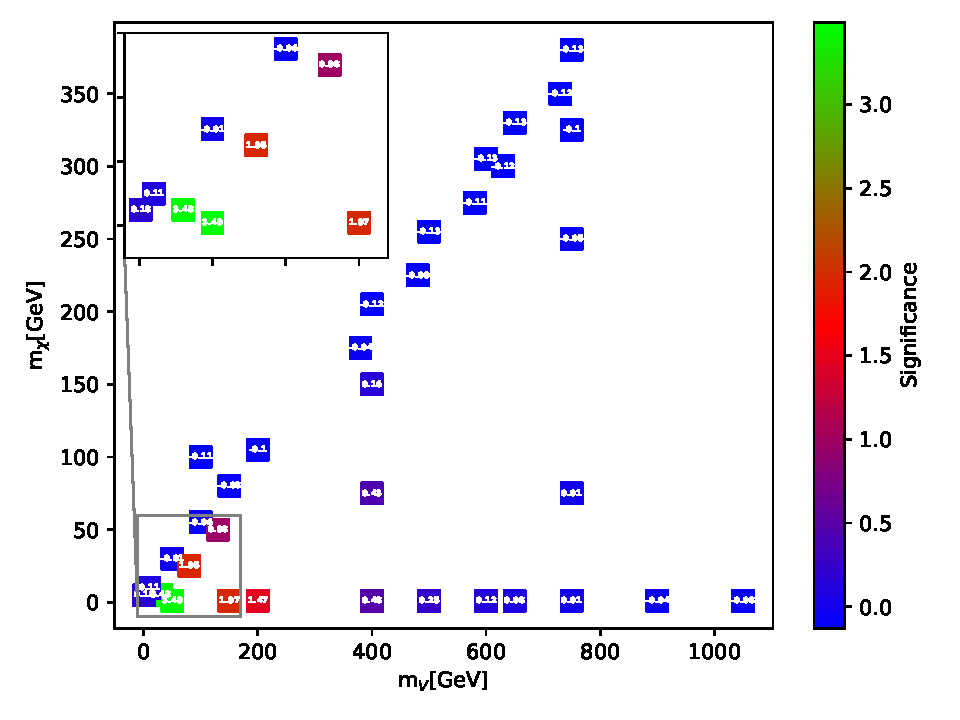
\includegraphics[width = \textwidth]{Figures/Significances/significanceCutandCount_monoZ_all.pdf}
    \caption{Caption}
    \label{fig:my_label}
\end{figure}



\begin{figure}
    \centering
    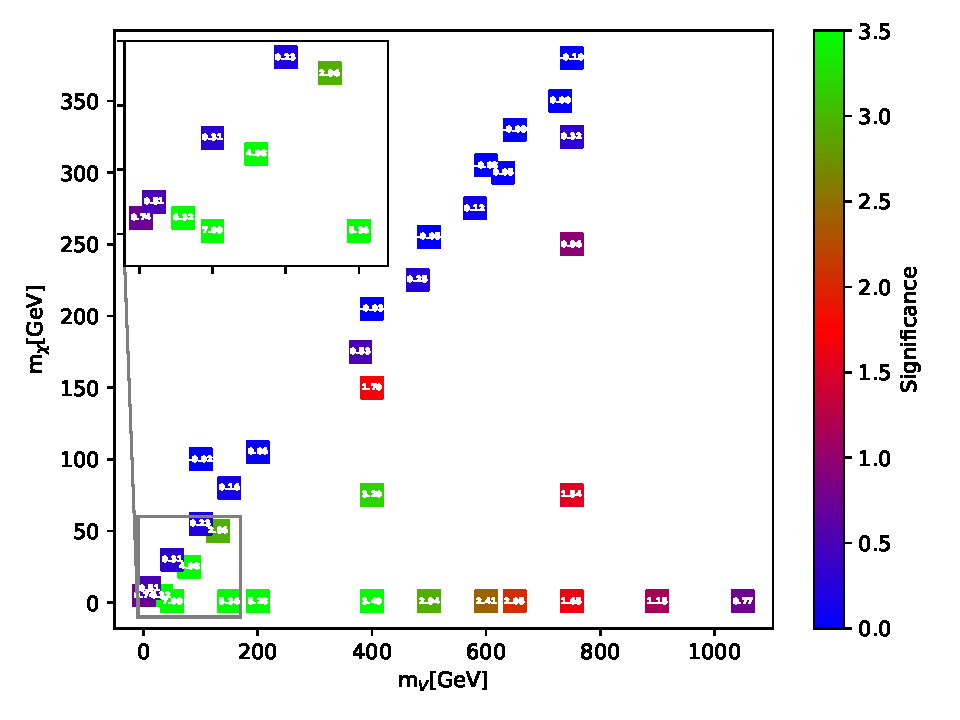
\includegraphics[width = \textwidth]{Figures/Significances/significance_BDT_monoZ_All_level.pdf}
    \caption{Caption}
    \label{fig:my_label}
\end{figure}

\begin{figure}
    \centering
    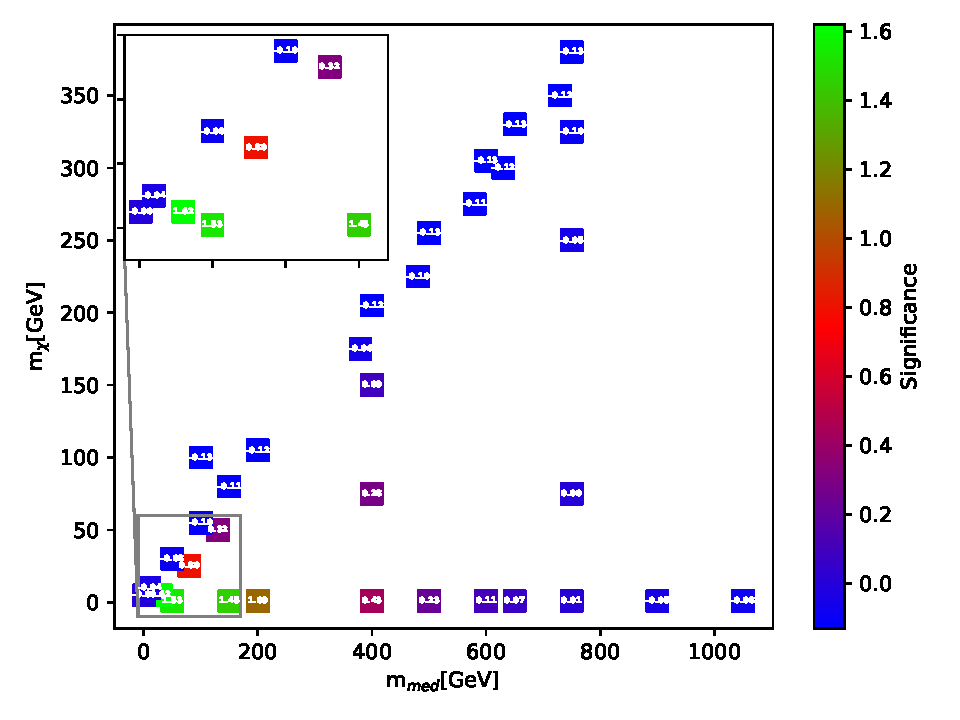
\includegraphics[width = \textwidth]{Figures/Significances/significance_BDT_monoZ_Low_level.pdf}
    \caption{Caption}
    \label{fig:my_label}
\end{figure}


\begin{figure}
    \centering
    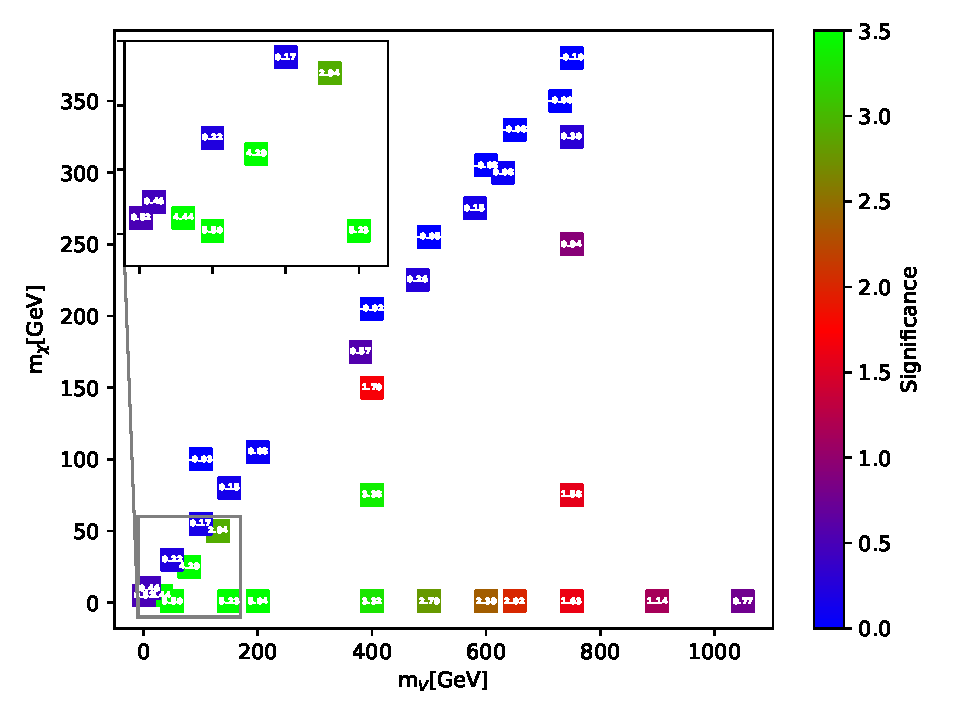
\includegraphics[width = \textwidth]{Figures/Significances/significance_BDT_monoZ_High_level.pdf}
    \caption{Caption}
    \label{fig:my_label}
\end{figure}



\begin{figure}
    \centering
    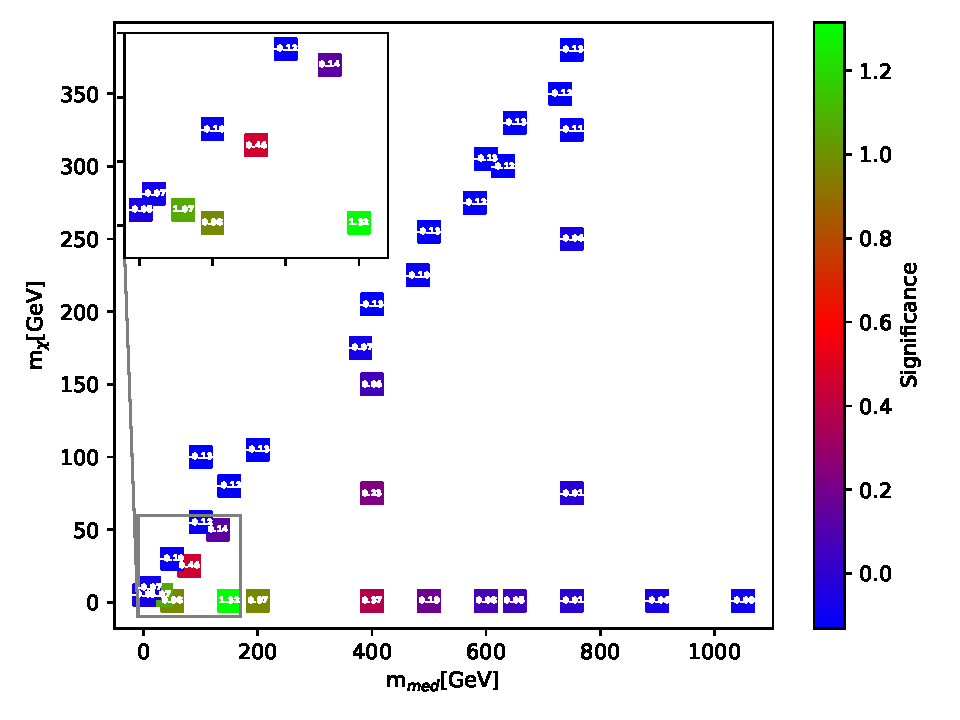
\includegraphics[width = \textwidth]{Figures/Significances/significance_NN_monoZ_All_level.pdf}
    \caption{Caption}
    \label{fig:my_label}
\end{figure}

\begin{figure}
    \centering
    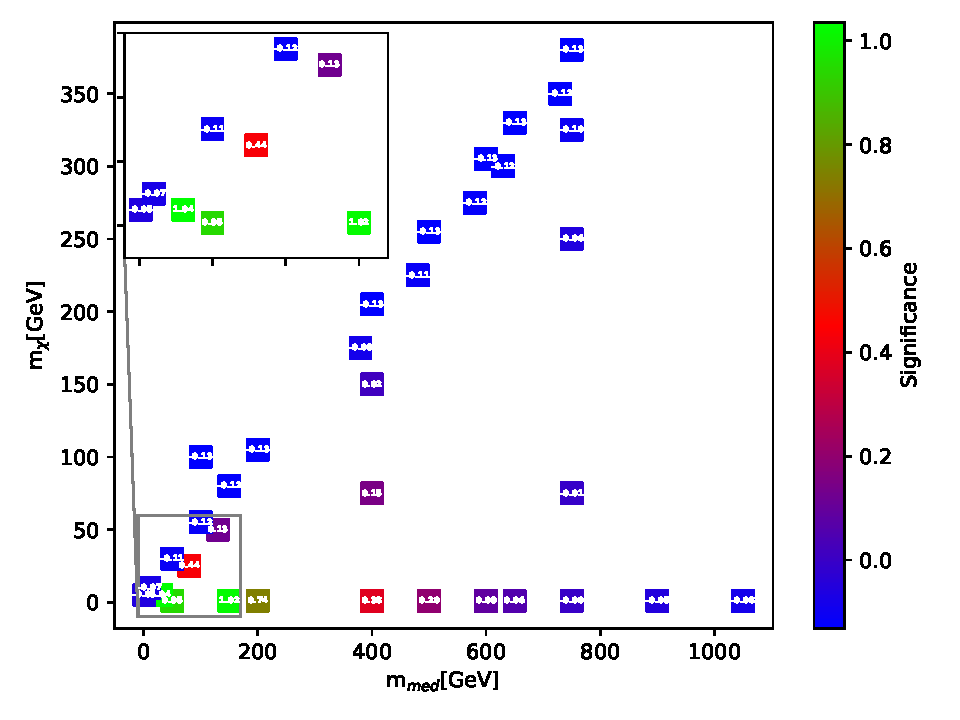
\includegraphics[width = \textwidth]{Figures/Significances/significance_NN_monoZ_Low_level.pdf}
    \caption{Caption}
    \label{fig:my_label}
\end{figure}


\begin{figure}
    \centering
    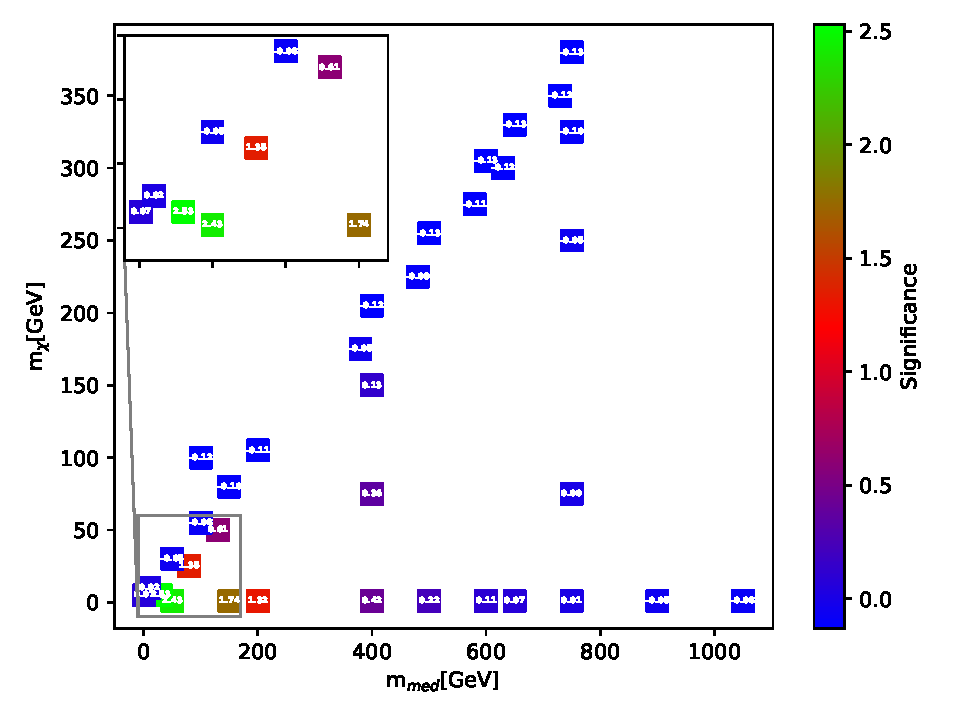
\includegraphics[width = \textwidth]{Figures/Significances/significance_NN_monoZ_High_level.pdf}
    \caption{Caption}
    \label{fig:my_label}
\end{figure}















